%% This is an example first chapter.  You should put chapter/appendix that you
%% write into a separate file, and add a line \include{yourfilename} to
%% main.tex, where `yourfilename.tex' is the name of the chapter/appendix file.
%% You can process specific files by typing their names in at the 
%% \files=
%% prompt when you run the file main.tex through LaTeX.
\chapter{Geometric Programming}

Sizing long-endurance aircraft for the stated requirements was accomplished using geometric programming. 

\section{Properties of Geometric Programs}

Geometric programs (GPs) are a mathematical optimization problem characterized by the convexity of the objective and constraint functions.\cite{gp} GPs have the form

\begin{align} 
\label{e:gpform}
\text{minimize } f_0(\bm{x}) & \nonumber \\
\text{subject to  } f_i(\bm{x}) &\leq 1, i=1,\ldots,m \\
g_i (\bm{x}) &= 1, i = 1,\ldots,p 
\end{align}

where the functions $g_i$ must be \emph{monomial} functions and the functions $f_i$ must be \emph{posynomial} functions. \emph{Monomials} and \emph{posynomials} have the forms

\begin{align}
 \label{e:mon}
g(\bm{x}) &= c x_1^{a_1} x_2^{a_2} \dotsm x_n^{a_n} , \\
\label{e:pos}
f(\bm{x}) &= \displaystyle\sum_{k=1}^K c_k x_1^{a_{1_k}} x_2^{a_{2_k}} \dotsm x_n^{a_{n_k}}.
\end{align}

The properties of a geometric program allow solution algorithms to guarantee convergence to a global optimum, provided that there exists a feasible solution to the set of constraint functions.  
Additionally, geometric programs can be solved rapidly with existing algorithms.  
Using state of the art, standard interior-point algorithms, GPs with 1,000 variables and 10,000 constraints converge to a solution in tens of seconds.\cite{gp}  

\section{Geometric Program Utilization}

To evaluate the gas and solar-electric powered aircraft design space, the requirements, architecture type, physical models, and assumed parameter values are expressed as constraints on the GP.\cite{hoburgthesis} 
Essentially, the gas and solar-electric powered geometric programs are long lists of constraints in a GP-form that can be solved using interior point methods.  
Figure~\ref{f:flowchart} shows how the optimization problem is constructed and solved. 
The following sections explain in detail the configuration, physical modeling, and input value assumptions and their resulting constraint equations that were used in both the gas and solar-electric powered optimization models.

\begin{figure}[h!]
	\begin{center}
	\includegraphics[width=1.0\textwidth,natwidth=568,natheight=154]{flowchart.eps}
    \caption{Process of constructing and solving a GP optimization problem.}
	\label{f:flowchart}
	\end{center}
\end{figure}

A python package for defining and manipulating geometric programs, GPkit\cite{gpkitdocs}, is used to create the models described in this paper.  
A commercial solver, mosek,\cite{mosek} is used to solve the GP. 
Both the gas and solar-electric powered GP optimization models are available for download and use.\cite{gassolartrade} 
